%Created with command:
%"/home/josh/Teaching/trunk/Utilities/makeexam" "Exam 1" "Please complete each problem.  Show all of your work even if you cannot obtain the correct answer.  You may use only a single sheet of letter sized paper for assistance." "../NumberSystems/Assessments/convert_binary_decimal_ex.tex" "../NumberSystems/Assessments/convert_hex_oct_bin_ex.tex" "../NumberSystems/Assessments/convert_hex_decimal_ex.tex" "../NumberSystems/Assessments/twos_complement_ex.tex" "../NumberSystems/Assessments/twos_complement_arithmetic_ex.tex" "../CMOSCircuits/Assessments/cmos_OR_gate_design.tex" "../CMOSCircuits/Assessments/dc_noise_margin_ex.tex" "../CombinationalCircuits/Assessments/simplify_logic_functions_ex.tex" "../CombinationalCircuits/Assessments/kmaps_ex.tex" "../CombinationalCircuits/Assessments/circuit_design_ex.tex"
\documentclass{article}
\usepackage[T1]{fontenc}
\usepackage{arev}
\usepackage{longtable}
\usepackage[hmargin=2cm,vmargin=2cm]{geometry}
\usepackage{graphicx}
\setlength{\parindent}{0pt}
\title{Exam 1}
\date{}
\begin{document}
\maketitle
Please complete each problem.  Show all of your work, even if you cannot obtain the correct answer.  You may use only a single sheet of letter sized paper for assistance. (40 points total)
\begin{longtable}[l]{rp{17cm}}
%file: ../NumberSystems/Assessments/convert_binary_decimal_ex.tex
1.&\begin{minipage}[t]{\linewidth}(2 pt) Convert the following binary numbers to decimal. \\
\\
(a) $11100001_2$ \\
(b) $0001.101_2$ \\

\vspace{4cm}
\end{minipage}\\
\medskip
%file: ../NumberSystems/Assessments/convert_hex_oct_bin_ex.tex
2.&\begin{minipage}[t]{\linewidth}(4 pt) Perform the following number system conversions. \\
\\
(a) $00101011_2 = ?_{16}$ \\
(b) $163_{16} = ?_8$ \\

\vspace{4cm}
\end{minipage}\\
\medskip
%file: ../NumberSystems/Assessments/convert_hex_decimal_ex.tex
3.&\begin{minipage}[t]{\linewidth}(2 pt) Convert the following hexadecimal number to decimal. \\
\\
$19\textrm{CA}_{16}$ \\

\vspace{4cm}
\end{minipage}\\
\medskip
%file: ../NumberSystems/Assessments/twos_complement_ex.tex
4.&\begin{minipage}[t]{\linewidth}(2 pt) Find the eight bit two's complement representation of each of the following numbers. \\
\\
(a) $-10$\\
(b) $-36$

\vspace{4cm}
\end{minipage}\\
\medskip
%file: ../NumberSystems/Assessments/twos_complement_arithmetic_ex.tex
5.&\begin{minipage}[t]{\linewidth}(6 pt) Perform the following binary arithmetic using the four bit two's complement representation, showing all carries.  For each case, determine if overflow occurs. If it does, state why it occurs.
\\
\\
(a) $4 - 3$\\
(b) $5 + -1$\\

\vspace{4cm}
\end{minipage}\\
\medskip
%file: ../CMOSCircuits/Assessments/cmos_OR_gate_design.tex
6.&\begin{minipage}[t]{\linewidth}(4 pt) Write the function table and draw the circuit diagram for a two input CMOS OR gate.  Note that this gate should use six transistors.\\ \\

\vspace{12cm
}
\end{minipage}\\
\medskip
%file: ../CMOSCircuits/Assessments/dc_noise_margin_ex.tex
7.&\begin{minipage}[t]{\linewidth}(2 pt) Given the following information from a data sheet, compute the HIGH and LOW state DC noise margins.\\ \\
$\textrm{V}_{\textrm{OHmin}} = 3.7 \textrm{V}$\\
$\textrm{V}_{\textrm{IHmin}} = 2.8 \textrm{V}$\\
$\textrm{V}_{\textrm{ILmax}} = 1.9 \textrm{V}$\\
$\textrm{V}_{\textrm{OLmax}} = 0.4 \textrm{V}$\\

\vspace{4cm
}
\end{minipage}\\
\medskip
%file: ../CombinationalCircuits/Assessments/simplify_logic_functions_ex.tex
8.&\begin{minipage}[t]{\linewidth}(6 pt) Using the theorems of switching algebra, simplify the following logic functions to a sum of of products representation.\\ \\
(a) $F=X' \cdot Y \cdot Z + Y \cdot X + X \cdot Y \cdot Z + Z \cdot X \cdot Y$ \\
(b) $F=Z \cdot (X' + Y') + X \cdot Y \cdot Z$ \\

\vspace{12cm
}
\end{minipage}\\
\medskip
%file: ../CombinationalCircuits/Assessments/kmaps_ex.tex
9.&\begin{minipage}[t]{\linewidth}(6 pt) Use a Karnaugh map to find a minimal sum of products represention of the following logic function.\\ \\
$F=\prod_{W,X,Y,Z}(6,7,8,9,10,11,12,13,14)$\\

\vspace{12cm
}
\end{minipage}\\
\medskip
%file: ../CombinationalCircuits/Assessments/circuit_design_ex.tex
10.&\begin{minipage}[t]{\linewidth}(6 pt) Design a digital logic circuit that accepts an unsigned three bit binary number as input and outputs a 1 if that number is either even or a power of 2.  Otherwise, the circuit outputs a 0.  Write a minimal sum of products representation of the logic function for the circuit.

\vspace{12cm
}
\end{minipage}\\
\medskip
\end{longtable}
\newpage
Axioms and theorems of switching algebra:\\ \\
\begin{tabular}{llll}
  (A1) & $X=0$ if $X \neq 1$ & (A1$'$) & $X=1$ if $X \neq 0$ \\
  (A2) & If $X=0$, then $X'=1$ & (A2$'$) & If $X=1$, then $X'=0$ \\
  (A3) & $0 \cdot 0 = 0$ & (A3$'$) & $1 + 1 = 1$ \\
  (A4) & $1 \cdot 1 = 1$ & (A4$'$) & $0 + 0 = 0$ \\
  (A5) & $0 \cdot 1 = 1 \cdot 0 = 0$ & (A5$'$) & $1 + 0 = 0 + 1 = 1$ \\
  (T1) & $X + 0 = X$ & (T1$'$) & $X \cdot 1 = X$\\
  (T2) & $X + 1 = 1$ & (T2$'$) & $X \cdot 0 = 0$\\
  (T3) & $X + X = X$ & (T3$'$) & $X \cdot X = X$\\
  (T4) & $(X')' = X$ & &\\
  (T5) & $X + X' = 1$ & (T5$'$) & $X \cdot X' = 0$\\
  (T6) & $X + Y = Y + X$ & (T6$'$) & $X \cdot Y = Y \cdot X$ \\
  (T7) & $(X + Y) + Z = X + (Y + Z)$ & (T7$'$) & $(X \cdot Y) \cdot Z = X \cdot (Y \cdot Z)$ \\
  (T8) & $X \cdot Y + X \cdot Z = X \cdot (Y + Z)$ & (T8$'$) & $(X + Y) \cdot (X + Z) = X + Y \cdot Z$ \\
  (T9) & $X + X \cdot Y = X$ & (T9$'$) & $X \cdot (X + Y) = X$ \\
  (T10)& $X \cdot Y + X \cdot Y' = X$ & (T10$'$) & $(X + Y) \cdot (X + Y')=X$ \\
\end{tabular}\\
\begin{tabular}{llll}
  (T11)& $X \cdot Y + X' \cdot Z + Y \cdot Z = X \cdot Y + X' \cdot Z$ & &\\
  (T11$'$) & $(X + Y) \cdot (X' + Z) \cdot (Y+Z) = (X + Y) \cdot (X' + Z)$ & &\\
  (T12)& $X + X + \cdots + X = X$ & &\\
  (T12$'$) & $X \cdot X \cdot \cdots \cdot X = X$ & &\\
  (T13)& $(X_1 \cdot X_2 \cdot \cdots \cdot X_n)' = X_1' + X_2' + \cdots + X_n'$ & &\\
  (T13$'$) & $(X_1 + X_2 + \cdots + X_n)' = X_1' \cdot X_2' \cdot \cdots \cdot X_n'$ & &\\
  (T14)& $[F(X_1, X_2, \ldots, X_n, +, \cdot)]' = F(X_1', X_2', \ldots, X_n', \cdot, +)$ & &\\
  (T15)& $F(X_1, X_2, \ldots, X_n)= X_1 \cdot F(1, X_2, \ldots, X_n) + X_1' \cdot F(0, X_2, \ldots, X_n)$ & &\\
  (T15$'$) & $F(X_1, X_2, \ldots, X_n) = [X_1 + F(0, X_2, \ldots, X_n)] \cdot [X_1' + F(1, X_2, \ldots, X_n)]$ & &\\
\end{tabular} \\ \\
Three and four variable Karnaugh maps:\\ \\
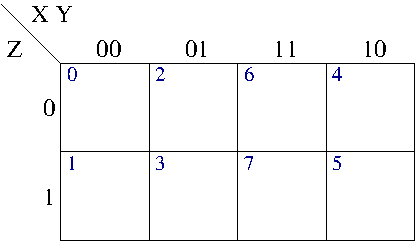
\includegraphics{../CombinationalCircuits/3VariableKMap}
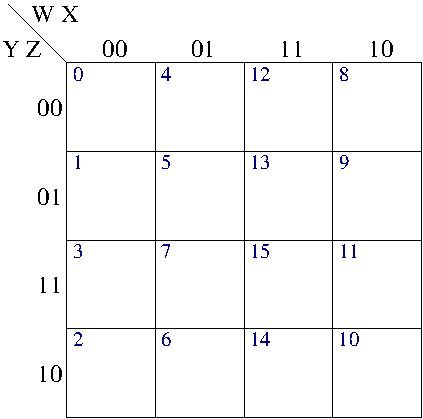
\includegraphics{../CombinationalCircuits/4VariableKMap}
\end{document}
